\section{dokumentation interpretation ergebnisse}
\label{sec:04_dokumentation_interpretation_ergebnisse}

Beide Modelle wurden nicht mittels einer Gridsearch optimiert, da durch die
sukssesive Veraenderung der Daten eine aufwendige suche der optimalen Parameter
notwendig waere.
Stattdessen wurde der Fokus auf eher robuste Modelle gelegt die resistente gegen
den Missmatch in den Daten sind.

Der Random Forest erwies sich bei kleinen Datensaetzen und sehr grossen
Missmatchen \SI{30}{\percent} als zuverlaessigeres Modell.
Trotz des Missmatches betrug die Accuracy \SI{50}{\percent}. 
Dies laesst sich darauf zurueckfuehren das der Missmatch mit der relativen
haeufigkeit der Klassen correliert ist. 
Zu den hauefigsten Klassen zaehlen die Klassen 'keine Wolken', 'stratocumulus',
'nimbostratus'. 
Diese weisen alle ein characteristisches Farbspektrum auf und sind einfach
anhand dessen von den anderen Klassen zu trennen.
Das training des CNN dagegen stellte sich als schwierig heraus. 
Trotz verschiedener Kernel-Groessen und anzahl an Convolutional Schichten lies
sich die Accuracy nicht wesentlich uber \SI{30}{\percent} anheben. 
Denkbar waere gewesen auf die Convolution zu verzichten und ebenso wie beim
Random Forest auf dem Farbspektrum zu trainieren.
Dies Methode erschien wesentlich einfacher zu regularisieren und den Missmatch
zu handeln.
Die Entscheidung viel jedoch bewust dagegen aus um das Verhalten des Neuronalen Netzes
auf schlecht simulierten Daten zu studieren. 

\begin{wrapfigure}{r}{0.6\textwidth}
		\centering
		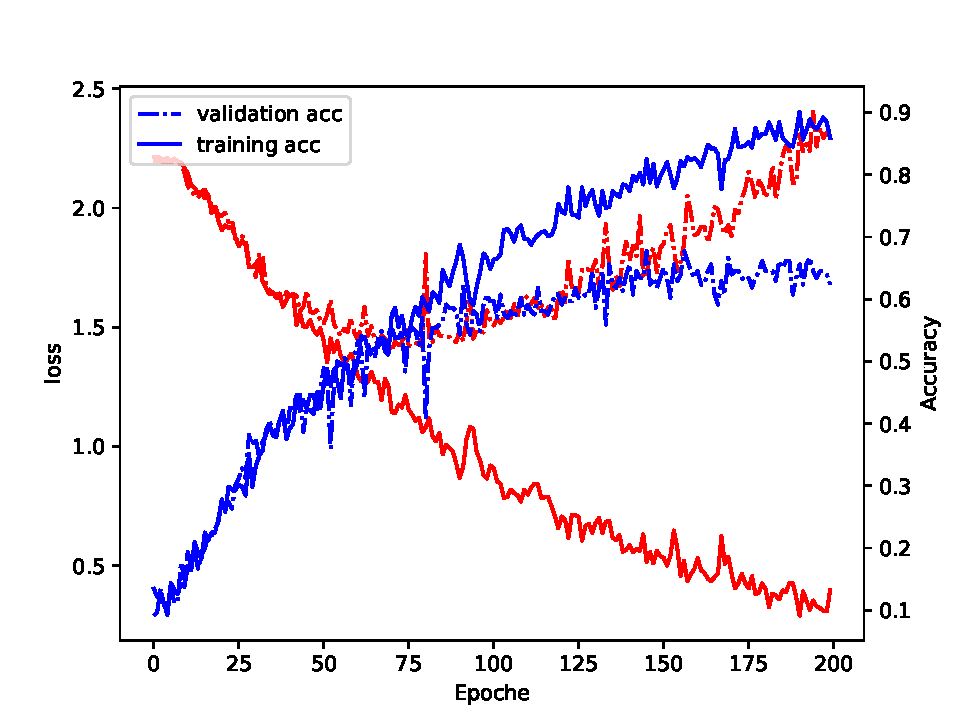
\includegraphics[width=0.6\textwidth]{pictures/train_nn.pdf}
		\caption{Loss sowie Accuracy in Abhaenigkeit der Trainingsepochen fuer
		Trainings sowie validierungsdaten.}
		\label{fig:}
\end{wrapfigure}
Der Random Forrest erreicht auf dem finalen Datensatz der immernoch einen
kleinen Missmatch enthaelt aus der uneindeutigkeit der Klassen und dem Fehler
des Bots eine ACC von \SI{62}{\percent}. 
Auf dem selben Test Datensatz zur evaluation betraegt die Accuracy des CNN
\SI{64}{\percent}.
Dabei ist die Accuracy abhaengig bei welcher Epoche der Schnitt zwischen Over-
und Underfitting macht.
Plausibel erscheint ein schnitt zwischen der \num{70} und \num{85} Epoche.
Auffaellig ist das der Validationloss anschliessend wieder Stark steigt und kein
Platto bildet.
Eine moegliche Ursache koennte der Missmatch seien.
In Abbildung \ref{fig:conf} sind die Confusion Matrizen der beiden Modelle
dargestellt. 
\begin{figure}[h]
		\centering
		\begin{subfigure}[b]{0.49\textwidth}
				\begin{center}
						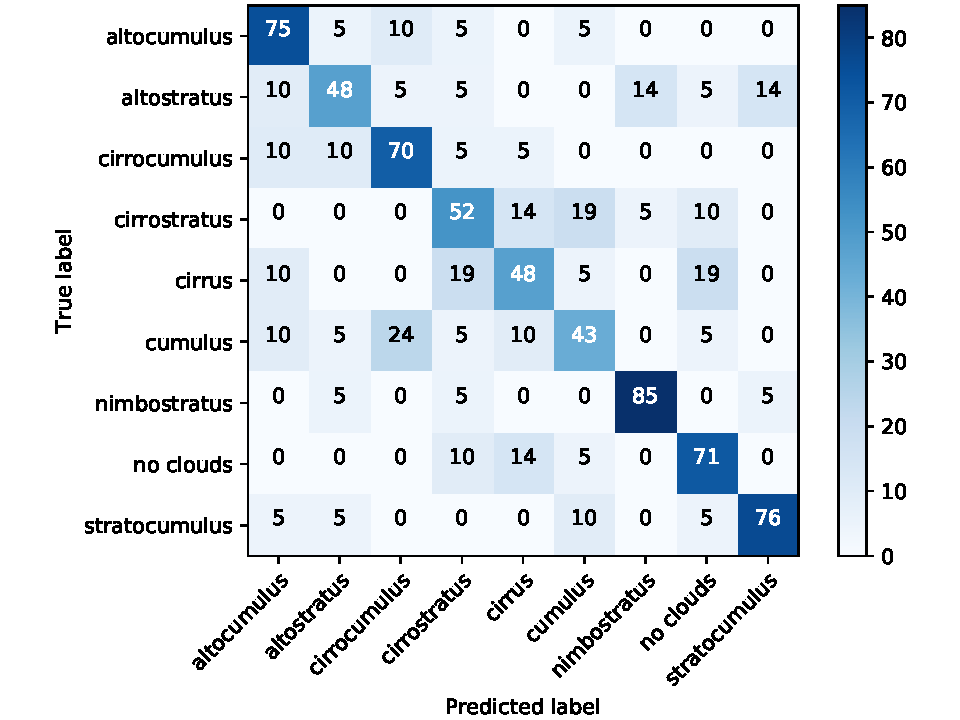
\includegraphics[width=\textwidth]{./pictures/conf_rf.pdf}
				\end{center}
				\caption{Random Forest}
				\label{fig:conf_rf}
		\end{subfigure}
		\begin{subfigure}[b]{0.49\textwidth}
				\begin{center}
						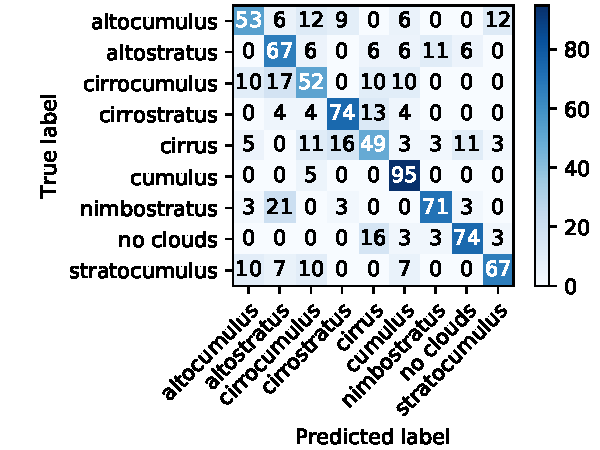
\includegraphics[width=\textwidth]{./pictures/conf_nn.pdf}
				\end{center}
				\caption{Convolutional Neuronal Network}
				\label{fig:conf_cnn}
		\end{subfigure}
		\caption{Konfidenz Matrizen der observierten Klassen bei denen das
		Vorhergesagte gegen das Wahre Klasse aufgetragen ist.}
		\label{fig:conf}
\end{figure}
Prinzipell scheinen der Random Forrest jeweils Probleme wenn das Farbspektrum
zweier Klassen sich nicht wesentlich unterscheidet.
Dies ist ueberwiegend dann der Fall wenn die Wolkenbedeckung des Himmels sich
Flaechenmaessig aehnelt. 
Beim CNN ist dies \ldots der Fall.

\begin{wrapfigure}{r}{0.32\textwidth}
		\centering
		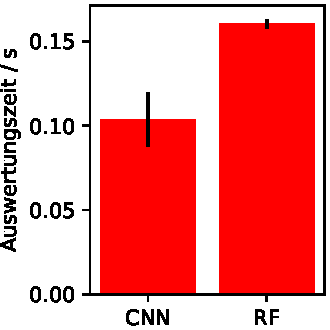
\includegraphics[width=0.3\textwidth]{pictures/time.pdf}
		\caption{Auswertungszeit auf Testdaten.}
		\label{fig:}
\end{wrapfigure}
keine Aussage ueber die Trainingszeit.
Zeitlicher vergleich der Methoden.
Wenn moeglich auch die Resourcen.

